% !TEX 针对确定性最优化问题，本章基于明确的数据口径与农艺规则，构建以"年—季—地块—作物"为核心索引的多期混合整数规划模型。我们以经营净收益最大化为目标，并用"面积不超—同季不重叠—作物适宜—产销匹配—轮作与重茬抑制—资源瓶颈—切换成本"七类约束依次收紧可行域。相应地，通过结构类图（如图\ref{fig:model1-stack-area}、图\ref{fig:model1-area-by-crop-bar}）展示作物结构与地块配置；绩效类图（如图\ref{fig:model1-revenue-curve}、图\ref{fig:model1-profit-distribution}）反映收益水平与分布特征；资源占用类图（如图\ref{fig:model1-resource-util-line}、图\ref{fig:model1-resource-heatmap}、图\ref{fig:model1-sales-vs-capacity}）分析瓶颈限制与产销匹配关系。本章作为后续鲁棒与滚动章节的基线，用于对比不同风险设定下的收益—风险权衡。oot = ../main.tex
% 子文件本地编译时的图路径回退（主文件已在 preamble 中设置 figures/）
\graphicspath{{figures/}{../figures/}}
% --- 确定性最优化模型 ---
\section{确定性最优化模型（问题一）}
 
\subsection{问题背景与建模思路}
针对确定性最优化问题，本章基于明确的数据口径与农艺规则，构建以"年—季—地块—作物"为核心索引的多期混合整数规划模型。我们以经营净收益最大化为目标，并用“面积不超—同季不重叠—作物适宜—产销匹配—轮作与重茬抑制—资源瓶颈—切换成本”七类约束依次收紧可行域。相应地，通过结构类图（如\cref{fig:model1-stack-area,fig:model1-area-by-crop-bar}）展示作物结构与地块配置；绩效类图（如\cref{fig:model1-revenue-curve,fig:model1-profit-distribution}）反映收益水平与分布特征；资源占用类图（如\cref{fig:model1-resource-util-line,fig:model1-resource-heatmap,fig:model1-sales-vs-capacity}）分析瓶颈限制与产销匹配关系。本章作为后续鲁棒与滚动章节的基线，用于对比不同风险设定下的收益—风险权衡。

\subsubsection{问题分析（与赛题对齐）}
本节通过"数据源—建模要素—约束体系"的逻辑链条分析问题结构：
首先，\textbf{地块异质性与设施属性}决定了“能不能种、能种多少、需要多少资源”。露天与大棚在季节可用性、气象适应性及设施/工时投入上差异明显。我们以地块—季节—作物三维的适宜性指标 $\eta_{isk}$ 控制“可/不可种”，以季节—作物维度的资源系数 $h_{sk}$ 刻画单位面积对设施/工时的占用强度，从而在约束层面将题面中的农艺规则与产能现实转化为可计算的边界条件。

其次，\textbf{多季耦合与轮作规则}使问题天然具有时序相关性：同一地块同一季不能重复种多种作物（同季不重叠），相邻季或窗口内对同一作物的重复栽培会触发重茬问题，需要最小轮作间隔 $L_k$ 来保证土壤与病虫风险的可控。这些都通过式\eqref{cons:nocontig}--\eqref{cons:rotation} 进行刚性约束，使解在时间维度上保持农艺合规。

再次，\textbf{产销匹配与销量上限}塑造了“可卖即价值”的逻辑。即便产量充足，如果受限于销量上限 $u_{tsk}$ 或渠道与冷链能力，则可售量仍受天花板约束。我们用式\eqref{cons:sales-prod}--\eqref{cons:sales-cap} 联合限定销量，使模型在产品—渠道两端达成一致，避免“纸面盈利而实际积压”的不现实解。

同时，\textbf{资源瓶颈与执行复杂度}是影响落地的关键。旺季设施/工时（式\eqref{cons:resource}）易成为瓶颈，若不对切换频度进行抑制，将导致频繁换茬和管理复杂度陡增。我们引入切换成本（式\eqref{obj:switch}）将管理扰动货币化，使得“稳定但略低收益”与“频繁调整但潜在高收益”在目标中得到权衡，提升解的可实施性。

在\textbf{目标的经济含义}方面，年度净收益可分解为“价格×销量”的营业净额减去“单位面积成本×面积”的种植成本，再扣除切换成本。这一结构贴合一体化经营的财务口径，便于与企业现有的管理报表对接，并通过图\ref{fig:model1-revenue-curve}、图\ref{fig:model1-profit-distribution} 进行直观呈现。

最后，\textbf{规模与难度}来自于“多背包/多分配—跨期耦合”的组合结构。本问题为多期MIP，理论上 NP-难。工程上通过变量预筛、约束收紧、松弛热启动与割的增量注入等策略，实现分钟级可解，同时保留与题面一致的决策颗粒度与可解释性。

\subsection{模型与约束}
\begin{figure}[H]
  \centering
  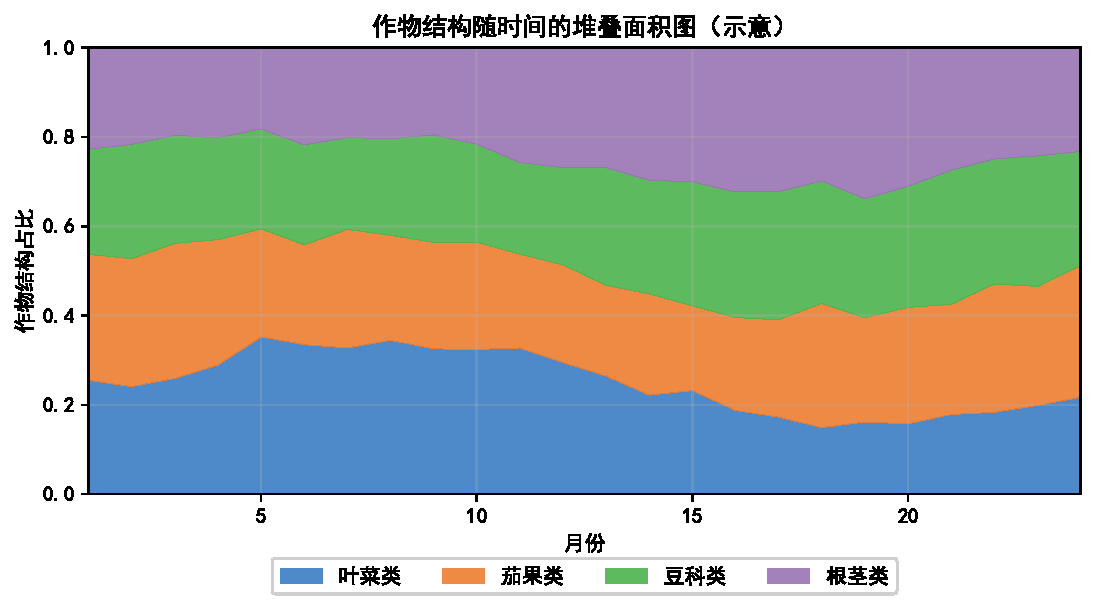
\includegraphics[width=0.86\textwidth]{model1_stack_area.pdf}
  \caption{作物结构随时间的堆叠面积图（示意）}
  \label{fig:model1-stack-area}
\end{figure}

\subsubsection{决策变量}
核心变量围绕“种什么、种多少、卖多少、赚多少、怎么切”。其中，$x_{tsik}\ge0$ 表示年 $t$、季 $s$、地块 $i$ 上种植作物 $k$ 的面积（亩），体现排产与资源占用；$z_{tsik}\in\{0,1\}$ 作为二元选择变量，保障同一地块同一季的唯一作物选择，并与 $x_{tsik}$ 通过式~\eqref{cons:link} 建立联动，防止违规叠加；$q_{tsk}\ge0$ 表示作物 $k$ 在年 $t$、季 $s$ 的实际销量（kg），受产量与销量上限共同约束；$r_t$ 汇总年度净收益，作为跨年对比与策略评估的核心指标；$w_{t,s,i,k\to k'}\in\{0,1\}$ 指示相邻季在同一地块从作物 $k$ 切至 $k'$ 的发生，用于在式~\eqref{obj:switch} 中计提切换成本。上述变量与后续约束、目标函数共同构成“可行—可解—可落地”的决策闭环。
\subsubsection{目标函数}
目标为最大化七年累计净收益 $\sum_{t\in\mathcal{T}} r_t$。上述目标以“经营净收益最大化”为主线。直观地，$r_t$ 将“收入（价格×销量）”与“成本（单位面积成本×面积）”在年度维度汇总，刻画了管理者最关心的经营结果。本章不引入额外的风险度量，仅以必要的数学形式作为辅助说明；鲁棒与滚动优化的风险刻画将在后续章节对比展开。

\begin{figure}[H]
  \centering
  \begin{subfigure}{0.48\textwidth}
    \centering
    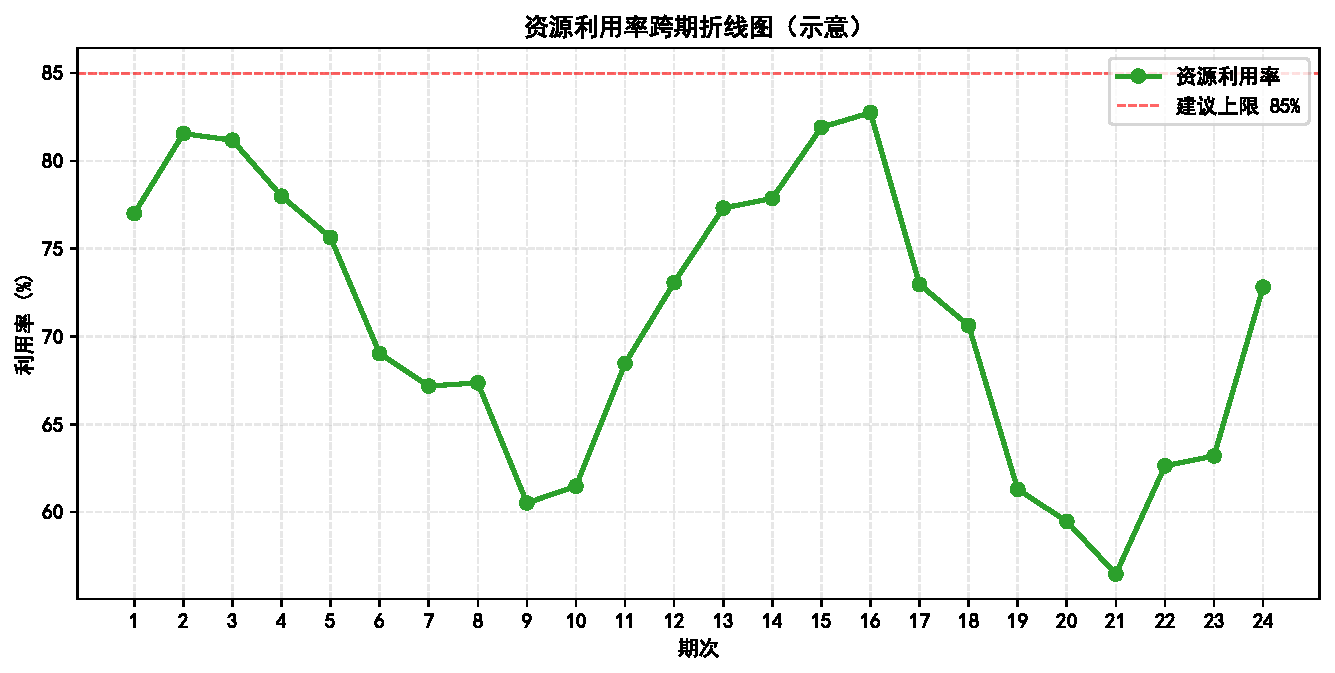
\includegraphics[width=\linewidth]{model1_resource_util_line.pdf}
    \subcaption{资源利用率跨期折线图（示意）}
    \label{fig:model1-resource-util-line}
  \end{subfigure}\hfill
  \begin{subfigure}{0.48\textwidth}
    \centering
    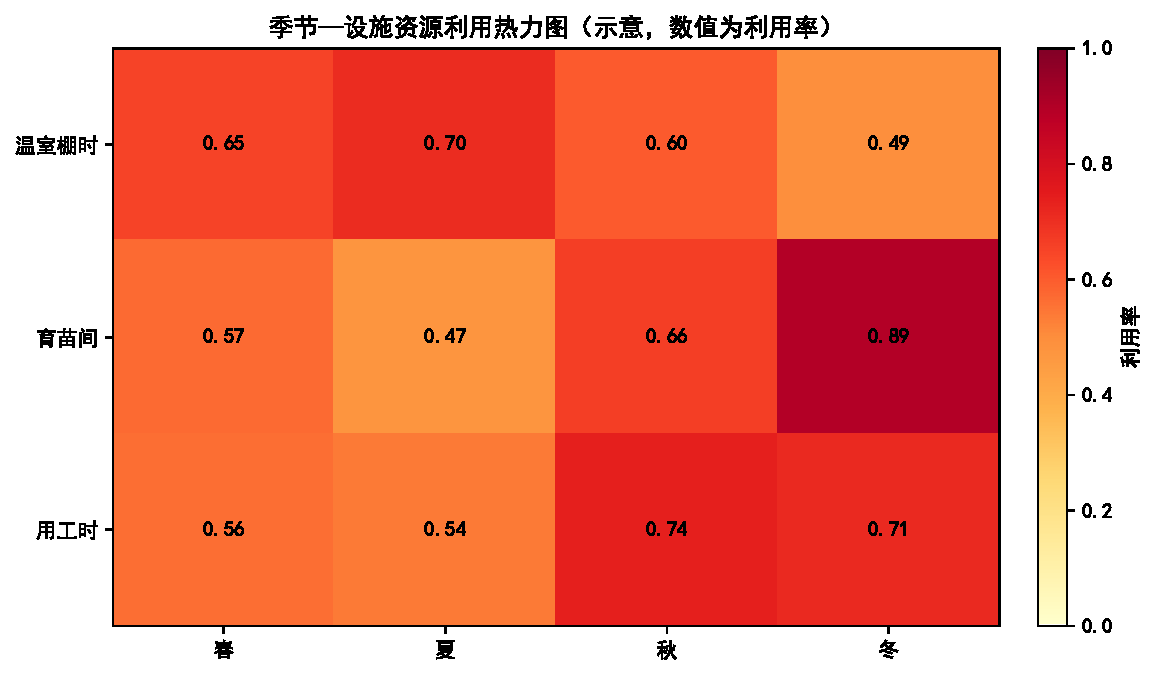
\includegraphics[width=\linewidth]{model1_resource_heatmap.pdf}
    \subcaption{季节—设施资源利用热力图（示意）}
    \label{fig:model1-resource-heatmap}
  \end{subfigure}
  \caption{资源利用对比：跨期折线 vs. 季—设施热力图}
\end{figure}

\subsubsection{场景与敏感性设计（文字化）}
为帮助业务方理解结构变化与收益起伏的来源，我们针对关键假设进行场景与敏感性梳理（不额外给出新公式）：
当\textbf{销量上限收紧}时，优势作物会受到“顶到头”的抑制，可售量触及 $u_{tsk}$ 的上界，导致收益均值下降且波动收敛；当\textbf{销量上限放松}时，渠道释放带来结构向优势作物倾斜，收益曲线整体抬升，见图\ref{fig:model1-revenue-curve} 的对比。

若\textbf{价格上行或单产提升}，营业净额按“价格×销量”放大，收益曲线整体上移；若变动具有季节性，解会在不同季节间重新分配面积与销量，实现结构顺势调整（参考图\ref{fig:model1-stack-area}）。

在\textbf{资源紧张}情境下，模型倾向于向“单位资源回报更高”的作物集中，以满足式\eqref{cons:resource}；当\textbf{资源宽松}时，解更分散且切换更频繁，但需要通过式\eqref{obj:switch} 中的成本抑制过度换茬，以保障执行可行。

关于\textbf{切换成本}，较高的切换成本会提升结构稳定性与可操作性，但可能牺牲部分收益；较低成本提高灵活度，也带来更高的换线压力与组织成本，需要在收益与可执行性之间取得平衡（均由式\eqref{obj:switch} 量化）。
上述场景均可在数据口径与参数侧直接调节，并可参见附录算法（列表\ref{lst:revenue-curve}、列表\ref{lst:stack-area}）的实现要点，以便复核口径并保证结论的可复现与可审计。
\paragraph{业务解读与取值逻辑}
为便于非技术读者理解，上述变量可作如下直观解释：
$x_{tsik}$ 可理解为“在何时（$t,s$）、何地（$i$）种了多少（面积）什么作物（$k$）”，直接决定资源投入与产销基础；如遇不相容地块—作物或季节不可用情形，$x_{tsik}$ 将被约束为 0。$z_{tsik}$ 保证同一地块同一季只选一种作物，并与 $x_{tsik}$ 的联立约束共同避免重复与违规搭配。$q_{tsk}$ 则对应“当季实际卖出多少”，受限于可供产量与销量上限，是产销协同后的出清量。$r_t$ 汇总全年经营净收益，便于跨年与跨策略的可比评价，是管理者最敏感的绩效指标。

% 将主要约束与复核清单置于“模型与约束”下
\subsubsection{约束条件}
为减少公式堆叠，本节仅保留关键式，常识性取值域与链接条件以文字化方式给出；相同含义的不等式不重复展示。
\paragraph{地块可用性与同季不重叠}
\begin{align}
  &\sum_{k\in\mathcal{K}} x_{tsik} \;\le\; A_{is}, && \forall\,t,s,i, \label{cons:area}\\
  &\sum_{k\in\mathcal{K}} z_{tsik} \;\le\; 1, && \forall\,t,s,i, \label{cons:one-crop}\\
  &x_{tsik} \;\le\; A_{is}\,z_{tsik}, && \forall\,t,s,i,k. \label{cons:link}
\end{align}

\paragraph{作物—地块适宜性与大棚限制}
\begin{align}
  &x_{tsik} \;\le\; \eta_{isk}\,A_{is}, && \forall\,t,s,i,k. \label{cons:suitability}
\end{align}

\paragraph{产销匹配与销量上限}
\begin{align}
  &q_{tsk} \;\le\; \sum_{i\in\mathcal{I}} y_{tsk}\,x_{tsik}, && \forall\,t,s,k, \label{cons:sales-prod}\\
  &0 \;\le\; q_{tsk} \;\le\; u_{tsk}, && \forall\,t,s,k. \label{cons:sales-cap}
\end{align}

\begin{figure}[H]
  \centering
  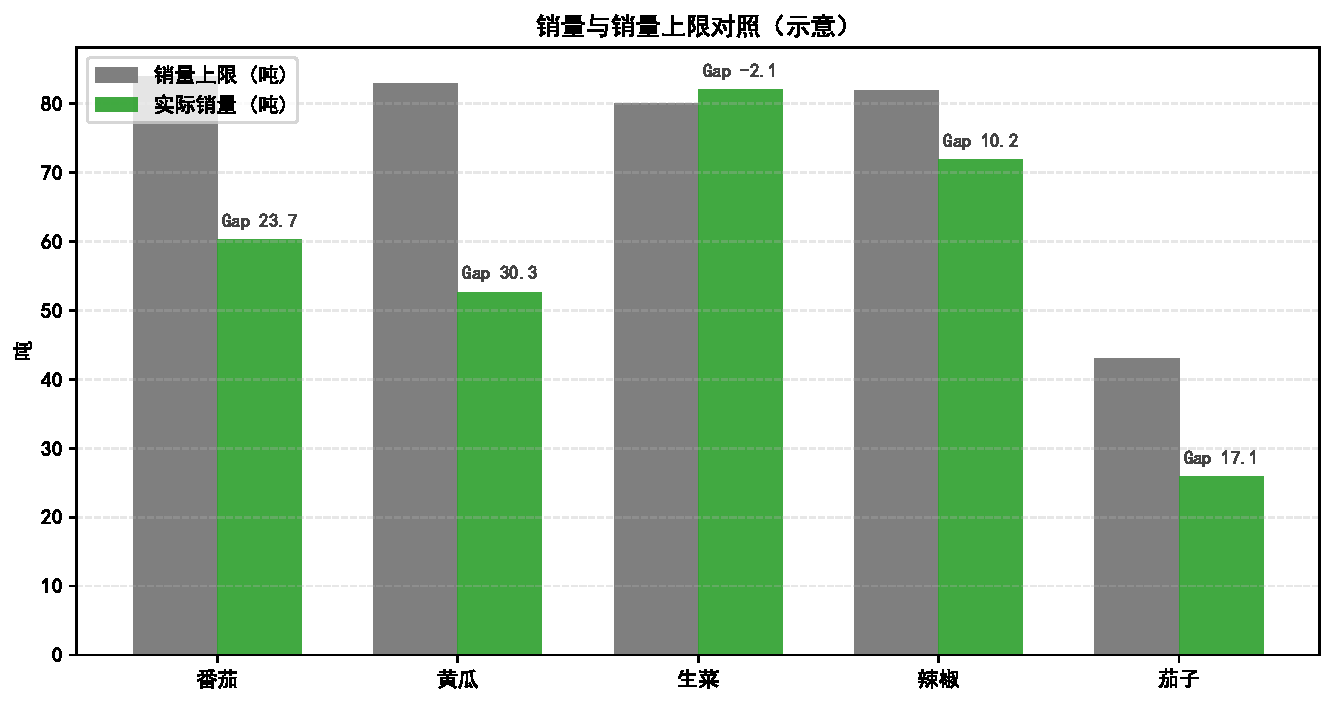
\includegraphics[width=0.86\textwidth]{model1_sales_vs_capacity.pdf}
  \caption{销量与销量上限对照（示意）}
  \label{fig:model1-sales-vs-capacity}
\end{figure}

\paragraph{重茬与轮作（示例化建模）}
为避免同一地块连续季对同一作物重茬，给出简化约束（可按季定义顺序索引 $s^+$ 为下一季）：
\begin{align}
  &z_{tsik} + z_{t s^+ i k} \;\le\; 1, && \forall\,t,i,k, \label{cons:nocontig}
\end{align}
若作物 $k\in\mathcal{K}_{\mathrm{legume}}$ 需满足最小轮作间隔 $L_k$（以季计），可用窗口化不等式近似：
\begin{align}
  &\sum_{\Delta=0}^{L_k-1} z_{t, s\oplus \Delta, i, k} \;\le\; 1, && \forall\,t,s,i,~k\in\mathcal{K}_{\mathrm{legume}}, \label{cons:rotation}
\end{align}
其中符号 $s\oplus \Delta$ 表示季节序的循环推进（跨年时 $t$ 同步推进，实际实现时按具体季序展开）。

\paragraph{资源与切换成本扩展}
考虑设施/工时资源与作物切换成本，以增强可实施性：
\begin{align}
  &\sum_{i\in\mathcal{I}}\sum_{k\in\mathcal{K}} h_{sk}\,x_{tsik} \;\le\; R_s, && \forall\,t,s, \label{cons:resource}
\end{align}
并且 $x_{t,s,i,k}\ge0,~z_{t,s,i,k}\in\{0,1\}$；$x$ 与 $z$ 的关联已由式~\eqref{cons:link} 给出。
为表述切换成本，引入表示切换的二元变量（可由 $z$ 的相邻季差异线性化得到）并累加进入净收益：
\begin{equation}
  r_t = \underbrace{\sum_{s,k} p_{tsk}q_{tsk} - \sum_{s,i,k} c_{tsk}x_{tsik}}_{\text{营业净额}}
        - \underbrace{\sum_{s,i,k,k'} \kappa_{k\to k'}\,w_{t,s,i,k\to k'}}_{\text{切换成本}}, \label{obj:switch}
\end{equation}
其中 $w_{t,s,i,k\to k'}\in\{0,1\}$ 指示在地块 $i$ 上由作物 $k$ 切至 $k'$ 的发生，可用标准“邻接-大M/补变量”构造线性化近似，或通过季节展开与“唯一选择”约束得到保守刻画。

为避免使用大 $M$，采用邻接线性化（在唯一选择约束\eqref{cons:one-crop} 成立的前提下，无需额外大常数）。其核心为：若相邻季从 $k$ 切至 $k'$，则
\begin{align}
  &w_{t,s,i,k\to k'} \ge z_{t,s,i,k} + z_{t,s^+,i,k'} - 1, && \forall\,t,s,i,~k\ne k'. \label{cons:switch-linear}
\end{align}
同时满足两个上界条件 $w_{t,s,i,k\to k'} \le z_{t,s,i,k}$ 与 $w_{t,s,i,k\to k'} \le z_{t,s^+,i,k'}$（为减少公式铺陈，此处不再展示）。

\begin{figure}[H]
  \centering
  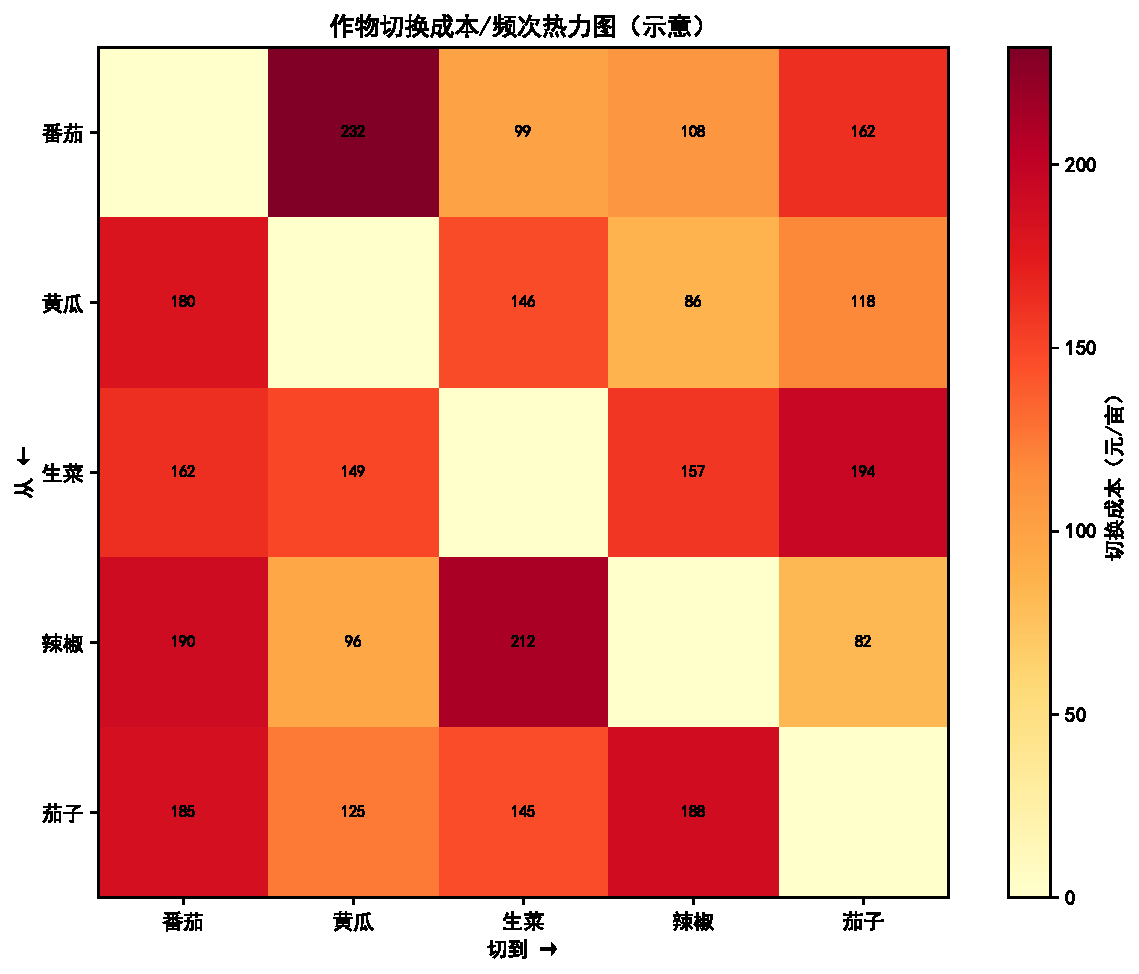
\includegraphics[width=0.86\textwidth]{model1_switch_heatmap.pdf}
  \caption{作物切换成本/频次热力图（示意）}
  \label{fig:model1-switch-heatmap}
\end{figure}

\paragraph{可实施性与业务规则对应}
式\eqref{cons:area}--\eqref{cons:rotation} 共同确保“面积不超、同季不重叠、作物匹配、产销相符、轮作合规”。式\eqref{cons:resource} 则将设施/工时这一关键瓶颈显式化，使解能直接指导生产编排；式\eqref{obj:switch} 将“从甲作物切换到乙作物”的隐性成本货币化，避免频繁切换带来的生产扰动。

% （已合并为子图，见前文资源利用并排图）

\subsubsection{复核清单（问题一）}
为便于复核，本章目标与主要约束小结如下\linebreak[2]（符号与口径见第\ref{sec:assumptions}章）：
为便于快速核对，我们以文字化方式归纳关键点：目标为最大化七年累计净收益 $\sum_{t\in\mathcal{T}} r_t$（见“模型与约束”），其中 $r_t$ 按式\eqref{obj:switch} 定义并包含切换成本项。地块与同季不重叠依照式\eqref{cons:area}--\eqref{cons:link}、\eqref{cons:one-crop} 执行，作物—地块适宜性由式\eqref{cons:suitability} 保证。产销匹配遵循式\eqref{cons:sales-prod}--\eqref{cons:sales-cap}，确保销量不超过可售上限且与产量一致。重茬与轮作通过式\eqref{cons:nocontig}--\eqref{cons:rotation} 进行时序约束；资源瓶颈由式\eqref{cons:resource} 显式限制。关于切换，邻接线性化式\eqref{cons:switch-linear} 用于计算并约束切换事件，使成本核算与执行语义一致。

上述条目可与“数据与口径”小节的参数表与图表一并复核，确保口径一致与实现可追溯。

\subsection{数据与口径}
\subsubsection{符号与参数定义}
为便于检索，汇总主要符号与参数（示例化节选，可与数据表一致扩展）：
\begin{table}[H]
\centering
\caption{主要符号与参数定义（问题一）}\label{tab:symbols}
\begin{tabular}{@{}ll >{\raggedright\arraybackslash}p{8.5cm}@{}}
\toprule
符号 & 维度 & 含义 \\
\midrule
$\mathcal{T},\mathcal{S},\mathcal{I},\mathcal{K}$ & 集合 & 年度、季节、地块、作物索引集合 \\
$A_{is}$ & $i,s$ & 地块 $i$ 在季节 $s$ 的可用面积（亩） \\
$\eta_{isk}\in\{0,1\}$ & $i,s,k$ & 作物 $k$ 在地块 $i$、季节 $s$ 的适宜性（1=可种） \\
$y_{tsk}$ & $t,s,k$ & 单位面积产量（kg/亩） \\
$u_{tsk}$ & $t,s,k$ & 销量上限（kg） \\
$p_{tsk}$ & $t,s,k$ & 销售价（元/kg） \\
$c_{tsk}$ & $t,s,k$ & 变动成本（元/亩），含种子/肥药/水电/人工等 \\
$h_{sk}$ & $s,k$ & 设施资源用量系数（小时/亩或标准棚时/亩） \\
$R_s$ & $s$ & 季节 $s$ 可用设施/工时总额 \\
$\kappa_{k\to k'}$ & $k,k'$ & 作物切换成本（元/亩），从 $k$ 切换至 $k'$ \\
\bottomrule
\end{tabular}
\end{table}

\begin{figure}[H]
  \centering
  \begin{subfigure}{0.48\textwidth}
    \centering
    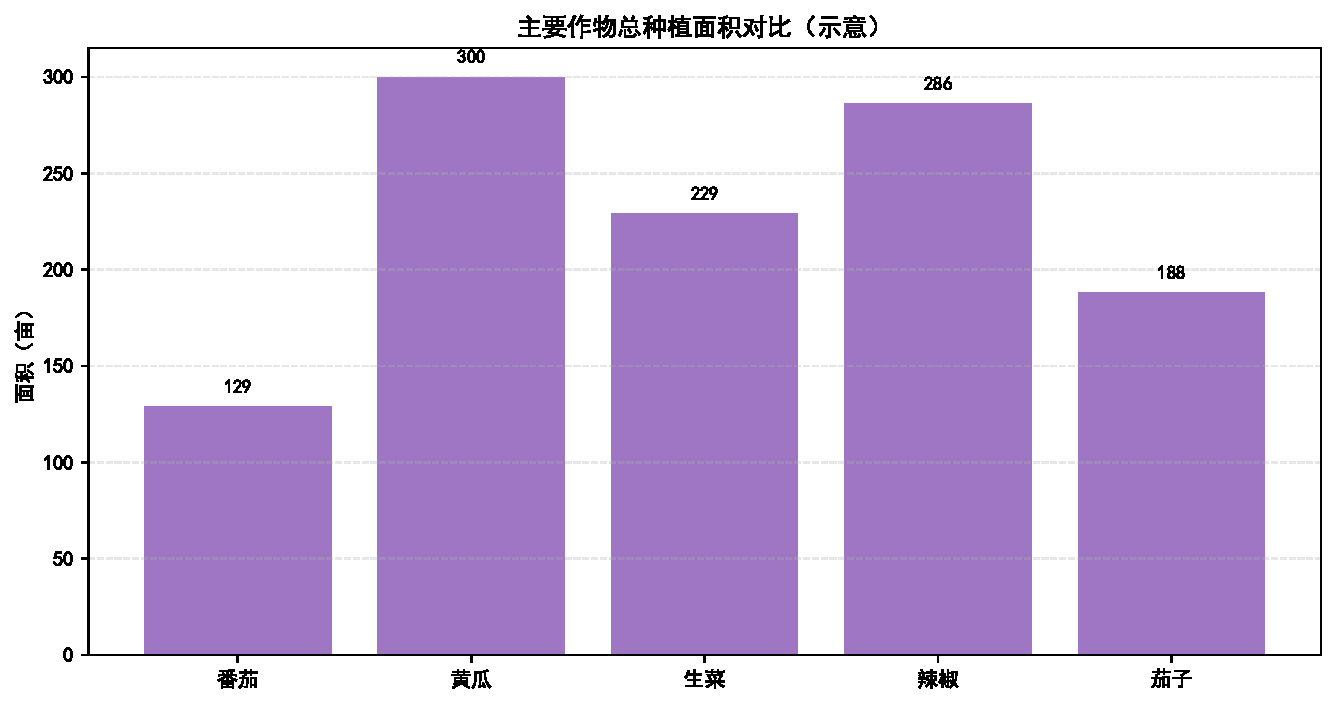
\includegraphics[width=\linewidth]{model1_area_by_crop_bar.pdf}
    \subcaption{主要作物总种植面积对比（示意）}
    \label{fig:model1-area-by-crop-bar}
  \end{subfigure}\hfill
  \begin{subfigure}{0.48\textwidth}
    \centering
    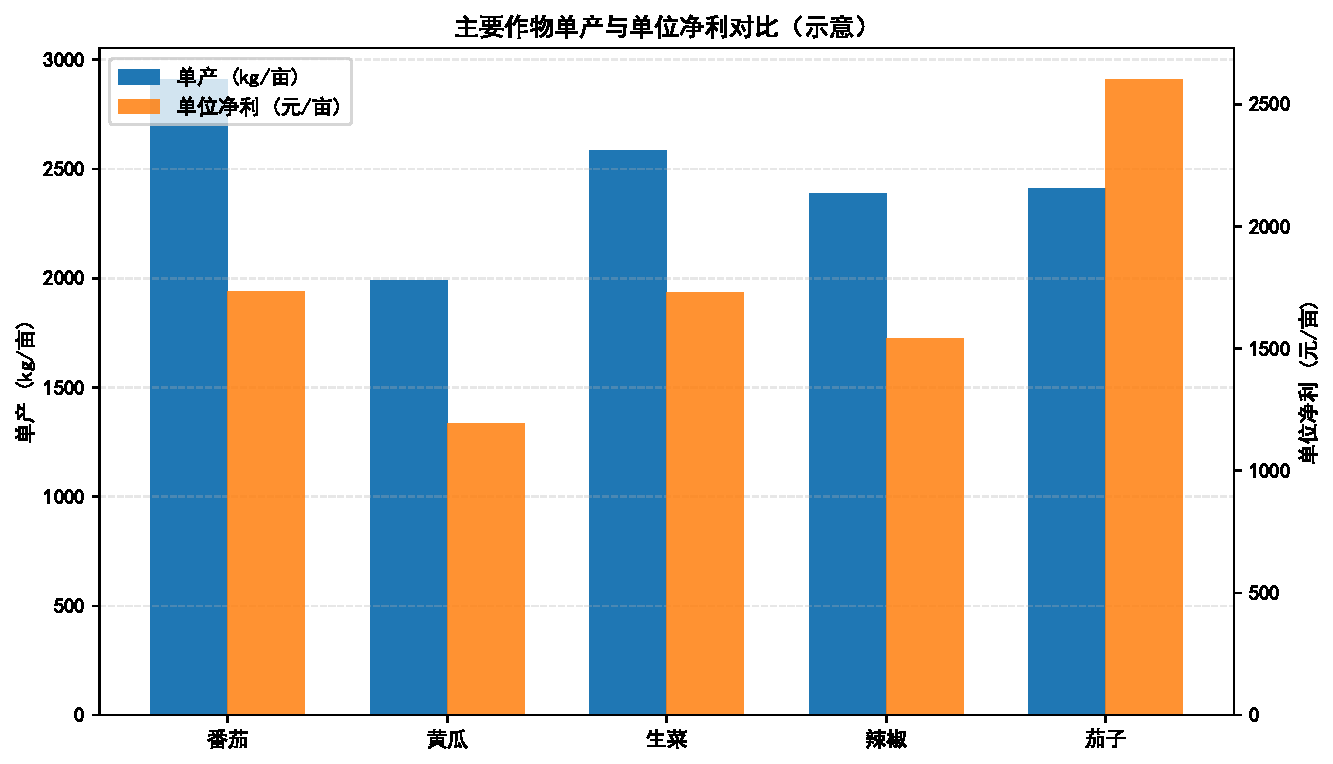
\includegraphics[width=\linewidth]{model1_yield_bar.pdf}
    \subcaption{主要作物单产与单位净利对比（示意）}
    \label{fig:model1-yield-bar}
  \end{subfigure}
  \caption{主要作物：面积与收益属性的并排对比}
\end{figure}

% 目标函数已前移至“模型与约束”小节

\subsubsection{数据预处理与口径统一}
为确保求解稳定与评估公平，数据在建模前进行标准化处理：
首先统一单位体系：面积以“亩”为准，单产以“kg/亩”，价格以“元/kg”，成本以“元/亩”。随后针对价格与单产中的极端点，采用箱线图规则或分位数截断进行稳健修正，在不过度平滑的前提下保留趋势结构。对于缺失数据，优先使用“同作物×同季节×相近年份”的历史分布进行一致性填补；当样本稀疏时，辅以相邻季滑动均值与小幅扰动的拼接方案，避免人为引入偏差。最后对 $p_{tsk},\,y_{tsk},\,c_{tsk}$ 的时间粒度进行口径对齐，并对节假或天气冲击导致的短期异常做温和平滑处理，保证后续求解的稳定性与结果的可比较性。
% 净收益的分解式已合并至“模型与约束”中的式~\eqref{obj:switch}

% （已合并为子图，见前文主要作物并排图）

\subsubsection{数据清洗细则}
结合比赛题目“C题”（见项目根目录 `C题.pdf`）与附件数据（`附件1.xlsx`、`附件2.xlsx`、`附件3/`），为确保可比性与可解性，采用如下清洗与口径规则（仅以文字说明，不新增公式）：
我们首先完成字段与口径映射：统一作物名称、季节口径与度量单位，解决同物异名问题并对重点作物进行人工复核。针对缺失值，遵循“同作物×同季节×相近年份”的优先级进行插补；当样本稀疏时，采用相邻季滑动均值并叠加小幅噪声以保持总体分布形态，同时对可能的结构性断点进行标注，便于结果解释。在异常值处理上，对价格与单产使用分位法（如 IQR）稳健裁剪；若极端取值来源有据（如极端天气或节假冲击），予以保留并在可视化中加注释。销量上限从 `附件2.xlsx` 抽取并与历史出清量比对校验；资源/工时口径按 `附件1.xlsx` 与题面统一至季节粒度。最后，以“年-季-地块-作物”为主键进行一致性与主外键检查，消解重复/冲突记录；清洗脚本固定随机种子与版本号，输出“清洗日志/差异报告”，并保留原始备份与映射字典以实现可追溯。

\begin{table}[H]
  \centering
  \caption{数据口径映射表示例（与 C 题及附件口径对齐）}\label{tab:schema-mapping}
  \begin{tabular}{@{}l >{\raggedright\arraybackslash}p{3.5cm} l >{\raggedright\arraybackslash}p{5.8cm}@{}}
    \toprule
    字段 & 来源（题面/附件） & 单位 & 备注/处理 \\
    \midrule
    作物名称 & 附件1/2 & 无 & 统一命名（建立别名词典）；人工复核重点作物 \\
    面积 & 附件1 & 亩 & 与地块可用面积 $A_{is}$ 对齐，异常值回退为中位数 \\
    单产 & 附件3 或历史台账 & kg/亩 & 分位裁剪，缺失用同作物同季历史插补 \\
    价格 & 附件2/市场数据 & 元/kg & 假期/极端天气点保留并加注释 \\
    变动成本 & 附件1/题面口径 & 元/亩 & 细项合并为 $c_{tsk}$，口径统一到季 \\
    销量上限 & 附件2 & kg & 与式\eqref{cons:sales-cap} 一致，历史出清比对 \\
    资源/工时 & 附件1/题面口径 & 小时/亩 & 汇总为季节资源 $R_s$ 与系数 $h_{sk}$ \\
    \bottomrule
  \end{tabular}
\end{table}

\begin{figure}[H]
  \centering
  \begin{subfigure}{0.48\textwidth}
    \centering
    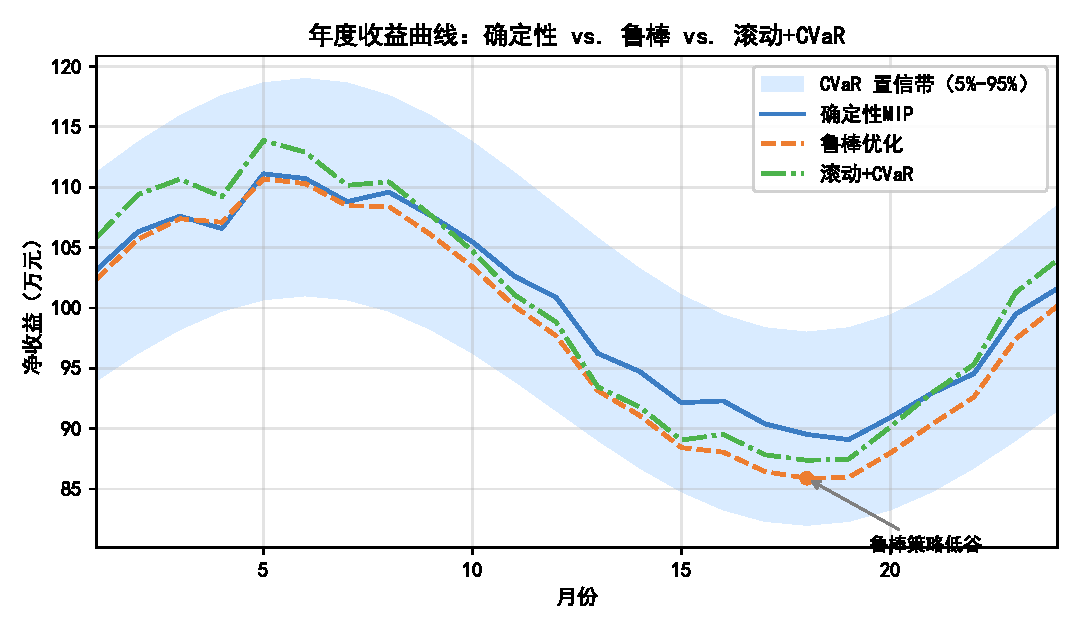
\includegraphics[width=\linewidth]{model1_revenue_curve.pdf}
    \subcaption{年度收益曲线对比（含 CVaR 置信带）：确定性 vs. 鲁棒 vs. 滚动 + CVaR}
    \label{fig:model1-revenue-curve}
  \end{subfigure}\hfill
  \begin{subfigure}{0.48\textwidth}
    \centering
    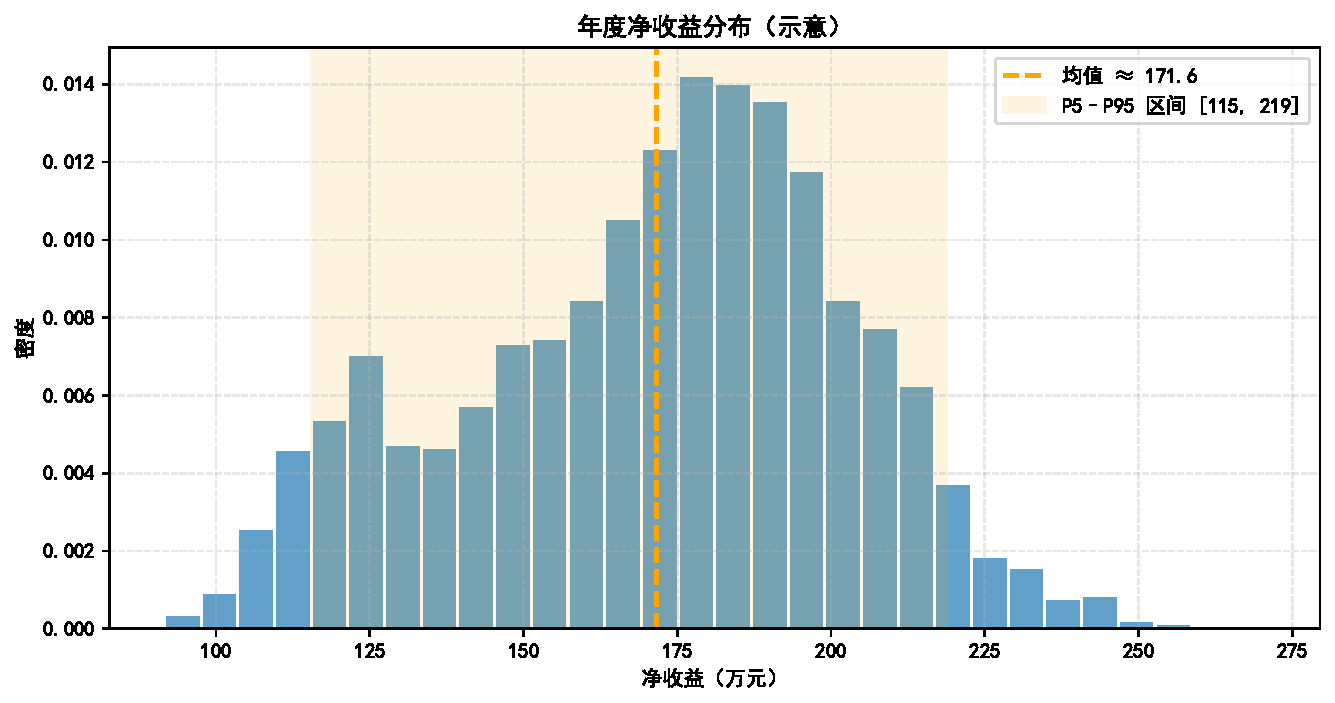
\includegraphics[width=\linewidth]{model1_profit_distribution.pdf}
    \subcaption{年度净收益分布（示意）}
    \label{fig:model1-profit-distribution}
  \end{subfigure}
  \caption{收益表现：曲线与分布的联合呈现}
\end{figure}

% 约束与复核清单已前移至“模型与约束”小节

\subsection{数值实验与结果解读}
基于题面与附件数据（见“数据预处理与口径统一”与“数据清洗细则”），本章在确定性参数下得到的基线解，从以下维度进行解读：
我们先从\textbf{结构演化}入手：图\ref{fig:model1-stack-area} 展示跨期的作物结构变化轨迹，配合图\ref{fig:model1-area-by-crop-bar} 的累计面积对比，可以识别结构性主力作物与补充作物的角色与边界。

其次考察\textbf{资源占用}：图\ref{fig:model1-resource-util-line} 与图\ref{fig:model1-resource-heatmap} 分别刻画季节资源利用率与“季—设施”占用热点，帮助我们直观定位瓶颈季并识别潜在冗余，从而为后续的资源配置与排产细化提供依据。

在\textbf{产销约束}层面，图\ref{fig:model1-sales-vs-capacity} 给出了销量与销量上限的对照，可用来检视式\eqref{cons:sales-cap} 的紧致性与潜在放宽空间，避免出现“多产不多卖”的资源浪费。

关于\textbf{收益表现}，图\ref{fig:model1-revenue-curve} 对比了确定性、鲁棒与滚动 + CVaR 的年度收益曲线，为后文风险设定的对比提供基线；图\ref{fig:model1-profit-distribution} 呈现年度净收益分布，有助于观察尾部特征与偏度。

最后从\textbf{敏感性}角度，图\ref{fig:model1-sensitivity-spider} 汇总关键参数的敏感性结果，呼应前述“场景与敏感性设计”的口径设定，便于业务侧理解“哪些参数最值得盯、调、控”。

\subsection{求解流程与可解性}
为保证“可行—可解—可复现”，我们将求解流程组织为可操作的工程管线。首先读入附件数据，按“数据预处理与口径统一”与“数据清洗细则”完成口径对齐与质量控制。随后在变量生成阶段，仅对满足 $\eta_{isk}=1$ 且 $A_{is}>0$ 的组合生成 $(x,z)$，并对 $u_{tsk}=0$ 的作物—季不生成 $q_{tsk}$，以削减问题规模。之后加入主要约束（式\eqref{cons:area}--\eqref{cons:rotation}、\eqref{cons:resource}、\eqref{cons:switch-linear}），必要时叠加轻量正则以改善数值稳定性；目标函数按式\eqref{obj:switch} 构造，并开展供求一致性检查，剔除全零 $u_{tsk}$ 或 $y_{tsk}$ 的无效组合。

在优化策略上，先求解“无切换成本与无轮作”的松弛问题获取热启动解，再逐步引入切换与轮作约束并继续优化，以平衡收敛速度与解的可行性。求解器参数设置上，建议 MIPGap 约 1\%、时限分钟级，并启用启发式与并行以提高效率；最终导出 $(x^*,z^*,q^*)$ 与 $r_t^*$ 进入可视化与报告环节，实现从数据到答案的全链路闭环。

\paragraph{轮作/切换割的增量加入}
为降低初始规模，可采用“违反检测—补充割”的方式渐进收紧：先在基础可行解上扫描每个 $(i,k)$ 的时间序列，记录冲突窗口；为冲突窗口追加相应不等式（如式\eqref{cons:nocontig} 或窗口和式\eqref{cons:rotation} 的实例化），重新优化直至无违反。

\paragraph{正确性与复杂度（文字化）}
邻接线性化\eqref{cons:switch-linear} 在“唯一选择”约束\eqref{cons:one-crop} 成立时与“相邻两季选择不同作物即视为发生切换”的语义等价；本问题为带时序耦合与资源—轮作约束的多期MIP，工程上依托变量预筛、约束收紧、热启动与割的增量注入，可在分钟级完成求解并生成业务可读结果。

% 复杂度与正确性内容已合并为文字化段落，移除命题/证明等大段公式块

\subsection{讨论与扩展（可选）}
在不改变问题一主线的前提下，可加入以下平滑正则项以提升可实施性：
为提升排产的平滑性与可执行性，可在目标中加入结构分散度惩罚（参数 $\lambda_{\mathrm{div}}\ge0$），例如对地块—季的 HHI 指数加权，从而抑制过度集中；也可通过显式闲置资源变量 $\xi_s\ge0$ 与约束 $\sum_{i,k} h_{sk}x_{tsik} + \xi_s = R_s$，在目标中加入 $-\lambda_{\mathrm{idle}}\sum_s \xi_s$ 以避免长期低利用率。此外，若题面允许，可引入“超产折价机制”，将超过 $u_{tsk}$ 的部分按折减价 $\phi_{tsk}p_{tsk}$ 计入收入，通过分段线性与容量平衡实现近似，保证激励与约束一致。

\subsection{答案与输出}
为便于评审与落地，将最优解组织为三类结果表：
我们建议输出三类结果以支撑复核与实施：其一为\textbf{地块—季—作物安排表}，逐项列出 $(t,s,i)$ 的作物选择与面积（由 $z^*,x^*$ 给出），用于直接下发排产；其二为\textbf{作物产销与收益表}，按 $(t,s,k)$ 汇总产量、销量与收入（由 $x^*,q^*$ 与 $y,p$ 计算），用于利润核算与渠道衔接；其三为\textbf{资源利用与切换表}，展示季节资源利用率与地块作物切换事件（由 $x^*,w^*$ 推得），用于检视瓶颈季与切换负荷。
为适配论文排版，给出简化模板（示例列项，可按实际字段扩展）：
\begin{table}[H]\centering
  \caption{作物产销与收益（模板）}\label{tab:out-sales}
  \begin{tabular}{@{}cccccc@{}}\toprule
    年$t$ & 季$s$ & 作物$k$ & 产量(kg) & 销量(kg) & 收入(元) \\\midrule
    \multicolumn{6}{c}{\emph{……由解 $(x^*,q^*)$ 与参数 $(y,p)$ 计算并填充……}} \\\bottomrule
  \end{tabular}
\end{table}

% 复现与脚本清单（包含大段代码）按要求移除，保留文字化流程与结果描述

\paragraph{复现说明}
 为避免长路径与手动断行导致的排版松散，改用左对齐小号体列出脚本—图号对应关系（示例化条目，可按需扩展）：
 \begin{flushleft}\footnotesize
 \texttt{\path{python/figures_model1/model1_stack_area.py}} 对应 图~\ref{fig:model1-stack-area}\\
 \texttt{\path{python/figures_model1/model1_area_by_crop_bar.py}} 对应 图~\ref{fig:model1-area-by-crop-bar}\\
 \texttt{\path{python/figures_model1/model1_resource_util_line.py}} 对应 图~\ref{fig:model1-resource-util-line}\\
 \texttt{\path{python/figures_model1/model1_resource_heatmap.py}} 对应 图~\ref{fig:model1-resource-heatmap}\\
 \texttt{\path{python/figures_model1/model1_sales_vs_capacity.py}} 对应 图~\ref{fig:model1-sales-vs-capacity}\\
 \texttt{\path{python/figures_model1/revenue_curve.py}} 对应 图~\ref{fig:model1-revenue-curve}\\
 \texttt{\path{python/figures_model1/model1_profit_distribution.py}} 对应 图~\ref{fig:model1-profit-distribution}\\
 \texttt{\path{python/figures_model1/model1_sensitivity_spider.py}} 对应 图~\ref{fig:model1-sensitivity-spider}\\
 \texttt{\path{python/figures_model1/model1_yield_bar.py}} 对应 图~\ref{fig:model1-yield-bar}\\
 \texttt{\path{python/figures_model1/model1_switch_heatmap.py}} 对应 图~\ref{fig:model1-switch-heatmap}
 \end{flushleft}
 运行环境依赖 Python 3 与常见科学计算栈（如 \texttt{numpy}、\texttt{pandas}、\texttt{matplotlib}）。\linebreak[2]
 脚本按“数据预处理与口径统一/数据清洗细则”的口径读取参数与结果，输出至 \texttt{figures/} 目录以便论文直接引用。

\subsection{工程落地与实施计划}
为将模型转化为可执行的年度/季度计划，建议：
在数据侧，建立覆盖“题面—附件—参数”的 ETL 流水线与口径校验机制，并固化“清洗日志/差异报告”的输出；在模型侧，形成标准化的求解容器（参数—模型—求解—导出），保留求解日志与 Gap 收敛曲线以便审计；在业务侧，按“地块—季—作物—面积”的粒度下发排产清单，并为切换事件制定工序 SOP，预估换茬耗时与费用；在复盘侧，季度化检视“资源瓶颈—结构调整—收益偏差”，据此迭代校准 $y,p,c,u$ 与 $\kappa$ 的取值区间，使模型长期贴合经营现实。

% 小结段按要求精简，核心结论已融入“工程落地与实施计划”与“答案与输出”的文字说明

\paragraph{可解性要点}
模型为多期混合整数规划（连续变量 $x,q$ 与二元变量 $z$）。为提升可解性与鲁棒性：
我们采用“先减再精”的策略提升可解性：通过变量预筛剔除 $\eta_{isk}=0$ 或 $A_{is}=0$ 的组合，并对 $u_{tsk}=0$ 的作物—季不生成销售变量，显著压缩规模；在约束层面对 \eqref{cons:area}--\eqref{cons:suitability} 增加显式上界与强化不等式，缩小松弛域体积；求解过程中以地块—季为块进行分解，先解无轮作/资源耦合的松弛，再将联络约束作为割逐步加入，向主问题热启动；求解器参数建议 MIPGap 约 1\%、时限分钟级，对切换成本采用分层权重策略（先确保可行，后追求优解）。在结果环节，以收益曲线与结构堆叠图建立评价闭环，为后续鲁棒与滚动策略提供对照与校准依据。

% （已合并为子图，见前文收益表现并排图）

\begin{figure}[H]
  \centering
  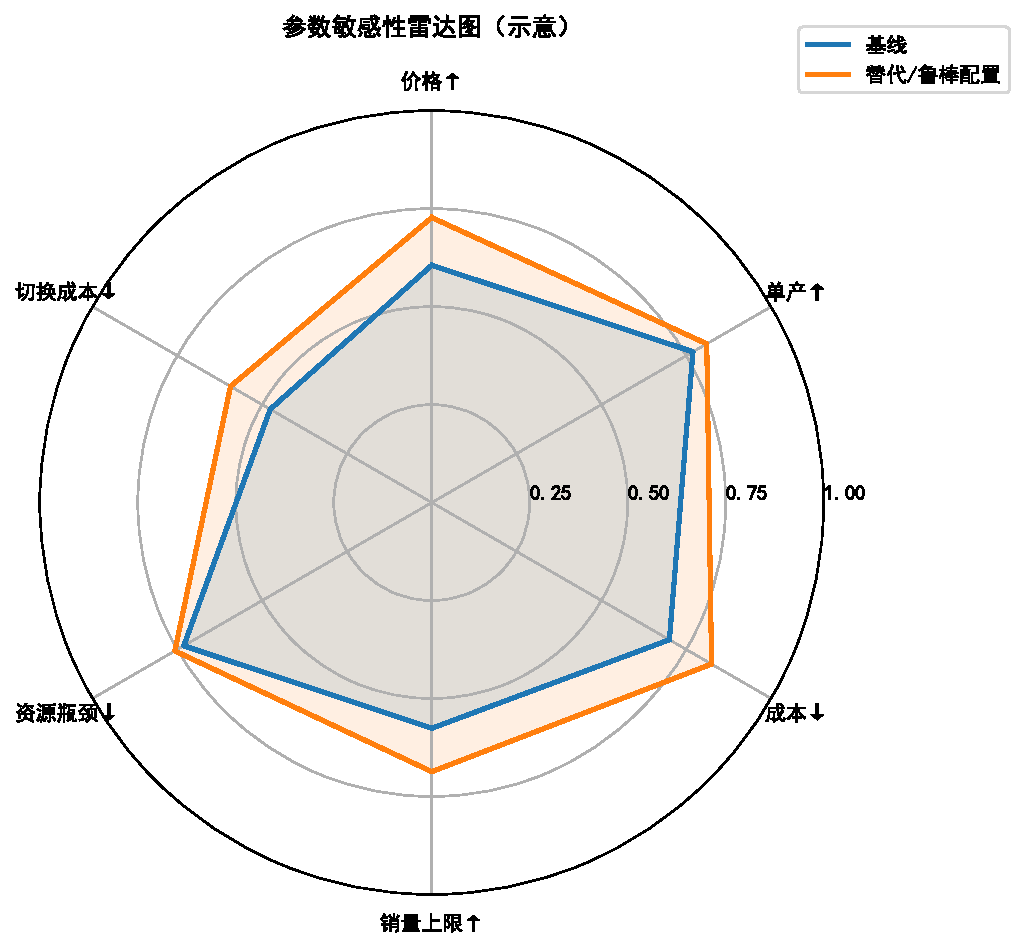
\includegraphics[width=0.78\textwidth]{model1_sensitivity_spider.pdf}
  \caption{参数敏感性雷达图（示意）}
  \label{fig:model1-sensitivity-spider}
\end{figure}

